\documentclass[table]{beamer}
\usepackage{lmodern}

\usepackage{etoolbox}
\usepackage{graphicx}
\usepackage{marginnote}
%\usepackage[usenames,dvipsnames]{color}
\usepackage[dvipsnames]{xcolor}
\usepackage{enumitem}

\usepackage{amssymb,amsmath}
\usepackage{ifxetex,ifluatex}
\usepackage{fixltx2e} % provides \textsubscript
\ifnum 0\ifxetex 1\fi\ifluatex 1\fi=0 % if pdftex
  \usepackage[T1]{fontenc}
  \usepackage[utf8]{inputenc}
\else % if luatex or xelatex
  \ifxetex
    \usepackage{mathspec}
    \usepackage{xltxtra,xunicode}
  \else
    \usepackage{fontspec}
  \fi
  \defaultfontfeatures{Mapping=tex-text,Scale=MatchLowercase}
  \newcommand{\euro}{€}
\fi
% use upquote if available, for straight quotes in verbatim environments
\IfFileExists{upquote.sty}{\usepackage{upquote}}{}
% use microtype if available
\IfFileExists{microtype.sty}{%
\usepackage{microtype}
\UseMicrotypeSet[protrusion]{basicmath} % disable protrusion for tt fonts
}{}
\ifxetex
  \usepackage[setpagesize=false, % page size defined by xetex
              unicode=false, % unicode breaks when used with xetex
              xetex]{hyperref}
\else
  \usepackage[unicode=true]{hyperref}
\fi
%\usepackage[usenames,dvipsnames]{color}
\hypersetup{breaklinks=true,
            bookmarks=true,
            pdfauthor={David Reinstein (Exeter)},
            pdftitle={},
            colorlinks=true,
            citecolor=blue,
            urlcolor=blue,
            linkcolor=magenta,
            pdfborder={0 0 0}}
\urlstyle{same}  % don't use monospace font for urls
\usepackage{graphicx,grffile}
\makeatletter
\def\maxwidth{\ifdim\Gin@nat@width>\linewidth\linewidth\else\Gin@nat@width\fi}
\def\maxheight{\ifdim\Gin@nat@height>\textheight\textheight\else\Gin@nat@height\fi}
\makeatother
% Scale images if necessary, so that they will not overflow the page
% margins by default, and it is still possible to overwrite the defaults
% using explicit options in \includegraphics[width, height, ...]{}
\setkeys{Gin}{width=\maxwidth,height=\maxheight,keepaspectratio}
\setlength{\parindent}{0pt}
\setlength{\parskip}{6pt plus 2pt minus 1pt}
\setlength{\emergencystretch}{3em}  % prevent overfull lines
\providecommand{\tightlist}{%
  \setlength{\itemsep}{0pt}\setlength{\parskip}{0pt}}
\setcounter{secnumdepth}{0}

\author{David Reinstein (Exeter)}
\date{25/09/2019}

% Redefines (sub)paragraphs to behave more like sections
\ifx\paragraph\undefined\else
\let\oldparagraph\paragraph
\renewcommand{\paragraph}[1]{\oldparagraph{#1}\mbox{}}
\fi
\ifx\subparagraph\undefined\else
\let\oldsubparagraph\subparagraph
\renewcommand{\subparagraph}[1]{\oldsubparagraph{#1}\mbox{}}
\fi

\begin{document}

\begin{frame}{Utility and Choice}
\protect\hypertarget{utility-and-choice}{}

(Largely from NS Chapter 2)

\end{frame}

\begin{frame}{Motivation}
\protect\hypertarget{motivation}{}

Consider a decision you recently made?

\bigskip

\begin{itemize}
\item
  Define this decision clearly.
\item
  How do you think you decided among these options?
\end{itemize}

2 minutes: discuss with your neighbour

What did this depend on? Would other people in your place have made the
same decision?

If you got amnesia and forgot what you decided and then were in the same
situation again. Do you think you'd make the same decision?

\end{frame}

\begin{frame}

Suppose I asked you

`State a rule that governs (determines/characterizes) how people
\emph{do} make decisions'\ldots{}

\bigskip

I want this rule to be\ldots{}

\begin{enumerate}
\item
  Informative (it rules \emph{out} at least some sets of choices)
\item
  Predictive (people rarely if ever violate this rule)
\end{enumerate}

\end{frame}

\begin{frame}

Similar question:

`State a rule that governs how people \emph{should} make decisions'..

\bigskip

By `should' I mean that \emph{they will not regret having made decisions
in this way.}

2 minutes: discuss with your neighbour

\end{frame}

\begin{frame}

\Huge If people \emph{did} follow these rules, what would this imply and
predict? \normalsize

Rules defined as `axioms about preferences'

`Standard axioms' \(\rightarrow\) (imply that) choices can be expressed
by `individuals maximising \emph{utility functions} subject to their
\emph{budget constraints}'

\(\rightarrow\) yields predictions for individual behavior, markets,
etc.

Economists and decision theorists have tried to come up with and defend
such rules.

They have started from these `reasonable axioms' and follow their
logical implications for \textCR individual choices, individual
responses to changes in prices and income,

market prices and quantities and their responses,

`welfare' and inequality outcomes for entire economies, etc.

\end{frame}

\begin{frame}{Lecture 2, Ch.2 -- Utility and Choice -- coverage}
\protect\hypertarget{lecture-2-ch.2-utility-and-choice-coverage}{}

\underline{Key goals of these lectures (and accompanying self-study)}

\textbf{Learn, understand, be able to explain and explain:}

\begin{itemize}
\item
  `Utility', how it's defined
\item
  Key assumptions about preferences/choices; their implications
\end{itemize}

\begin{itemize}
\tightlist
\item
  Depict preferences/utility with `indifference curves'

  \begin{itemize}
  \tightlist
  \item
    \ldots{} examples of `perfect substitutes' and `perfect complements'
  \end{itemize}
\end{itemize}

\end{frame}

\begin{frame}

\begin{itemize}
\tightlist
\item
  `Budget constraints', compute and model them
\end{itemize}

\begin{itemize}
\tightlist
\item
  Maximising utility subject to constraints

  \begin{itemize}
  \tightlist
  \item
    optimisation condition for this
  \end{itemize}
\end{itemize}

\begin{itemize}
\tightlist
\item
  Depict and interpret optimisation with indifference curves and budget
  constraints
\end{itemize}

Warn that this is somewhat abstract but it will make sense

Part 2 (ch 2-3) involves building the demand curve from first
principles,

and discussing how to interpret it

\begin{itemize}
\tightlist
\item
  Want to develop a model that can be used to show how we make choices
  or decisions.
\end{itemize}

-Your choices are determined by two things:

-Preferences: what goods do you like

-Constraints: how much money do you have, what are the prices of the
goods you buy

\end{frame}

\begin{frame}{Utility}
\protect\hypertarget{utility}{}

\begin{description}
\tightlist
\item[Utility]
``The pleasure or satisfaction that people get from their economic
activity.''
\end{description}

\begin{description}
\item[ \bigskip]
Alt: The thing that people maximise when making economic decisions
\end{description}

Adv: There is some debate about the meaning and interpretation of
utility, particularly in the Behavioural Economics literature

Adv: A defining feature of the standard Economics approach is that
decisions are made as if all characteristics of outcomes can be compared
and evaluated,

thus we can reduce everything to a single dimension, `utility', which is
maximised

\end{frame}

\begin{frame}

\emph{How is this used?}

\bigskip

Utility will be expressed as a single number that arises from the
combination of all goods and services consumed.

\bigskip

Essentially, economists assume that `when making a choice among all
available and feasible options, an individual will choose the one that
yields the greatest \emph{utility}'

\begin{block}{Utility from two goods}

\[Utility = U(X,Y; other)\]

\begin{itemize}
\tightlist
\item
  Leisure and `goods consumption'
\item
  Food and non-food
\item
  Coffee and tea (holding all else constant)
\end{itemize}

\end{block}

\end{frame}

\begin{frame}

\[Utility = U(X,Y)\]

\bigskip

\textcolor{blue}{Maths revision}: \(U(X,Y)\) expresses a \emph{function}
with two \emph{arguments}, X and Y.

\begin{itemize}
\tightlist
\item
  \(U(X,Y)\) must take \emph{some} value for every positive value of X
  and Y.
\end{itemize}

In \emph{general} a function of X and Y might increase or decrease in
either X or Y,

or increase over some ranges and decrease over other ranges of these two
arguments.

Consider the function `altitude of land in Britain as a function of
degrees longitude and latitude'

This expresses a \emph{general} function; I haven't specified
\emph{what} this function is

\begin{itemize}
\tightlist
\item
  E.g., it could be \(U(X,Y)=\sqrt(XY)\)
\end{itemize}

We can consider functions in general having certain properties without
specifying exactly what these functions are.

\begin{block}{Measuring and comparing utilities}

Adv: This is a difficult but well-studied issue, as it is important for
methodology and welfare analysis.

In more detailed discussions, we might speak of `cardinal utility',
`ordinal utility', etc.,

to indicate ways we can compare utility between individuals and in
response to policy changes.

Utility is not `observable and measurable in utils'

(Unlike midi-chlorians or thetans)

\bigskip

Utility is seen to govern an individual's \emph{choices} and thus it's
only inferred indirectly, from the \emph{choices} people make

\end{block}

\end{frame}

\begin{frame}

\textbf{Revealed preference:} if Al buys a cat instead of a dog, and a
dog was cheaper, we assume Al gets more utility from a cat

\begin{figure}

{\centering 
\includegraphics[width=0.9\linewidth]{picsfigs/alscat} 

}

\end{figure}

\end{frame}

\begin{frame}

\emph{Interpersonal comparisons are difficult}

\begin{itemize}
\tightlist
\item
  Who gets `more' utility?
\end{itemize}

\bigskip

\begin{figure}

{\centering 
\includegraphics[width=0.8\linewidth]{picsfigs/facepalmstatue} 

}

\end{figure}

\end{frame}

\begin{frame}

\emph{\ldots Interpersonal comparisons are difficult}

\begin{itemize}
\tightlist
\item
  Transfer from Al to Betty: Is the reduction in Al's utility more or
  less than the increase in Betty's?
\end{itemize}

\begin{figure}

{\centering 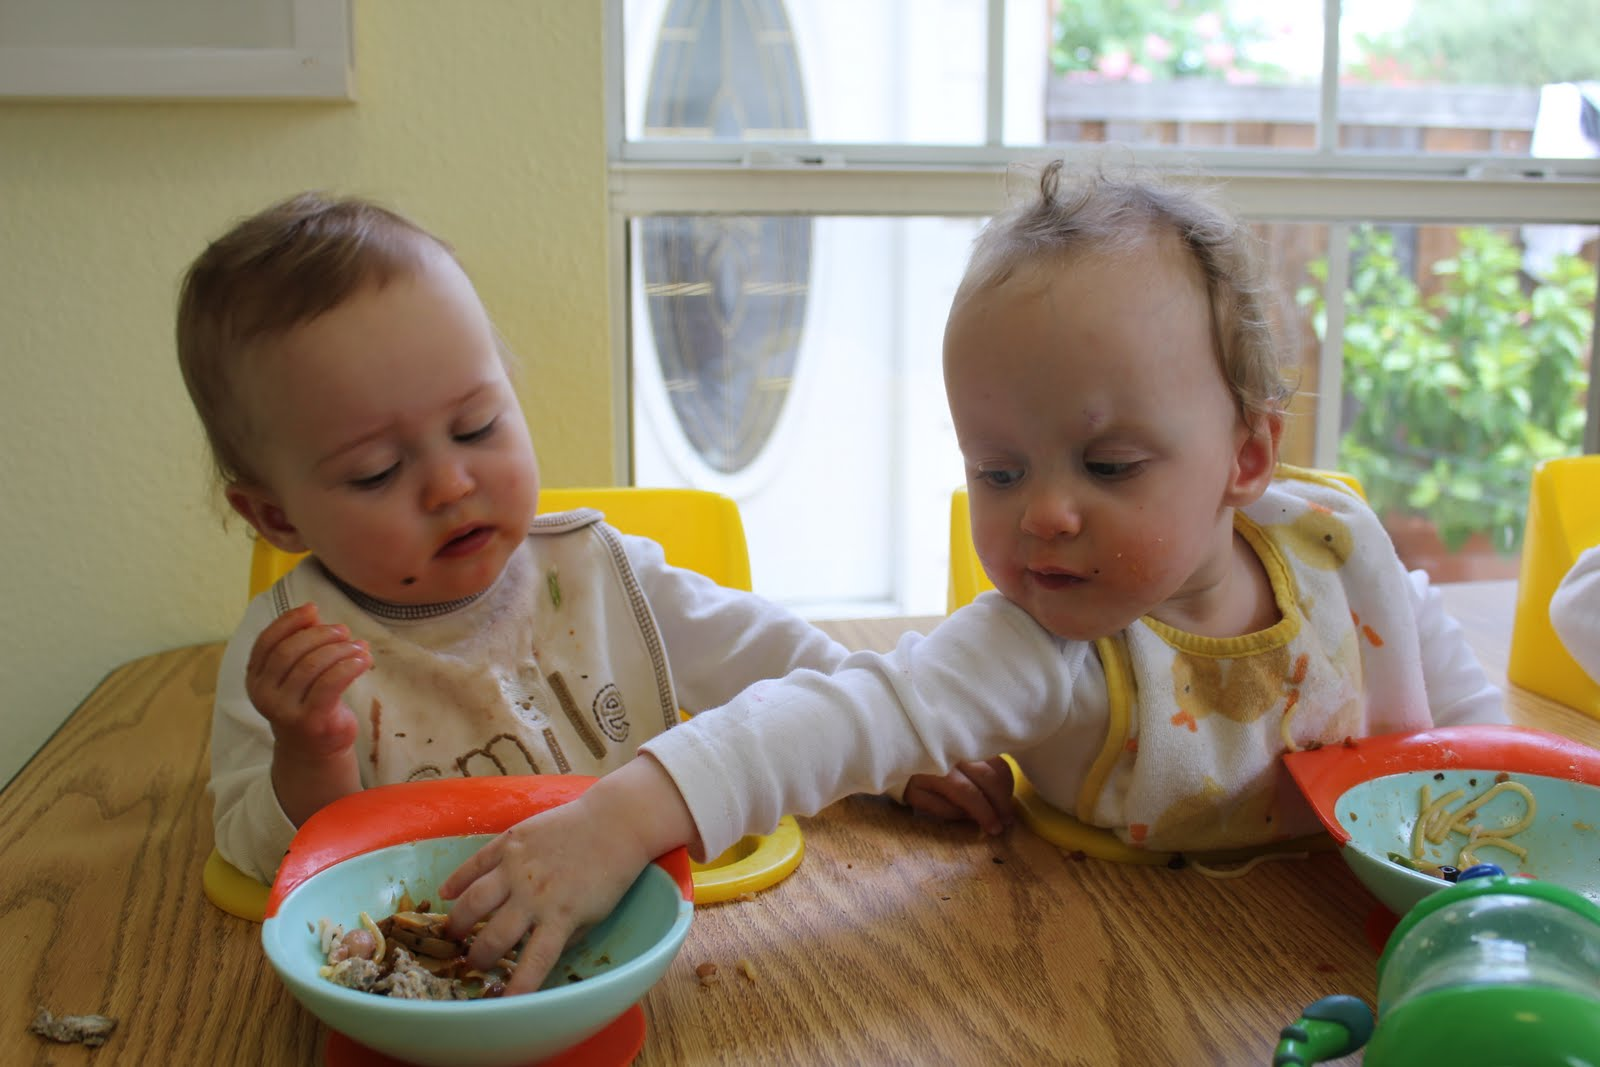
\includegraphics[width=0.9\linewidth]{picsfigs/babytakingfood} 

}

\end{figure}

As we only get at utility through an \emph{individual's} decisions, we
have no reliable way to compare it across individuals

\end{frame}

\begin{frame}{Standard assumptions about preferences (`axioms')}
\protect\hypertarget{standard-assumptions-about-preferences-axioms}{}

\begin{enumerate}
\tightlist
\item
  Completeness
\end{enumerate}

Given two options, A and B, a person can state which option they prefer
or whether they find both options equally attractive.

The more formal and parsimonious definition (Autor readings, Jehle/Reny)
develop this from a single relation `weakly preferred to'.

\begin{enumerate}
\setcounter{enumi}{1}
\tightlist
\item
  Transitivity (internal consistency)
\end{enumerate}

If I prefer A to B, and prefer B to C, then I must prefer A to C.

\begin{enumerate}
\setcounter{enumi}{2}
\tightlist
\item
  More is Better (\emph{nonsatiation})
\end{enumerate}

Completeness and transitivity (and continuity) are necessary for
people's choices to be represented by (continuous) \emph{utility
functions}

Continuity is necessary for `well behaved' (not-jumpy) demand curves

(Local) Nonsatiation will help us derive results

\end{frame}

\begin{frame}

\begin{block}{1. Completeness}

\[A \succ B, B \succ A, \: or \: A \sim B \]

\medskip

\textcolor{gray}{Fancy notation: Either A preferred to B, B preferred to A, or A indifferent to B}

You don't need to know this notation, but it may be a helpful shorthand

\begin{figure}

{\centering 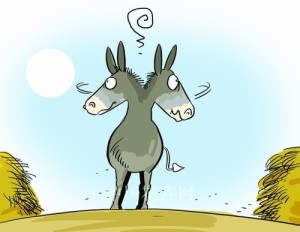
\includegraphics[width=0.5\linewidth]{picsfigs/donkeybales} 

}

\end{figure}

Forbidden: ``I can't choose between a ski holiday and a beach holiday,
but I am not indifferent''

Also forbidden: the \emph{time} or \emph{frame} in which I make the
\emph{decisions} shouldn't affect my choices

Violations?: See, e.g., 'Predicting Hunger: The Effects of Appetite and
Delay on Choice; Read and van Leeuwen, 1998

See also Sunstein and others on `choosing not to choose'

\end{block}

\end{frame}

\begin{frame}

\begin{block}{2. Transitivity}

\[ A \succ B \: and \: B \succ C \rightarrow A \succ C \]

\begin{itemize}
\tightlist
\item
  Similar for indifference (\(\sim\))
\end{itemize}

If I prefer an Apple to a Banana and a Banana to Cherry then I prefer an
Apple to a Cherry.

A similar idea holds if I am indifferent between one pair of these.

If this seems confusing it may be because it is \emph{too} obvious
(although behavioral and experimental economists claim to find
violations).

\end{block}

\end{frame}

\begin{frame}

\begin{figure}

{\centering 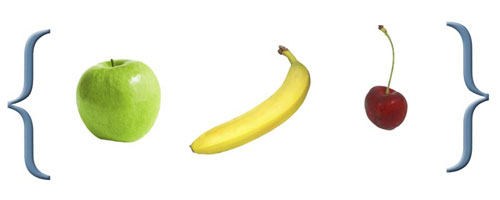
\includegraphics[width=0.5\linewidth]{picsfigs/applebananacherry} 

}

\end{figure}

If I prefer an Apple to a Banana and a Banana to Cherry

then I prefer an Apple to a Cherry.

If not \(\rightarrow\) money pump.

Adv: `Money pump' argument -- If you found someone who strictly
preferred an apple to a banana, a banana to a cherry, and a cherry to an
apple,

you could make a lot of money out of them!

\end{frame}

\begin{frame}

\begin{block}{3. More is better (similar to nonsatiation,
`monotonicity')}

\begin{figure}

{\centering 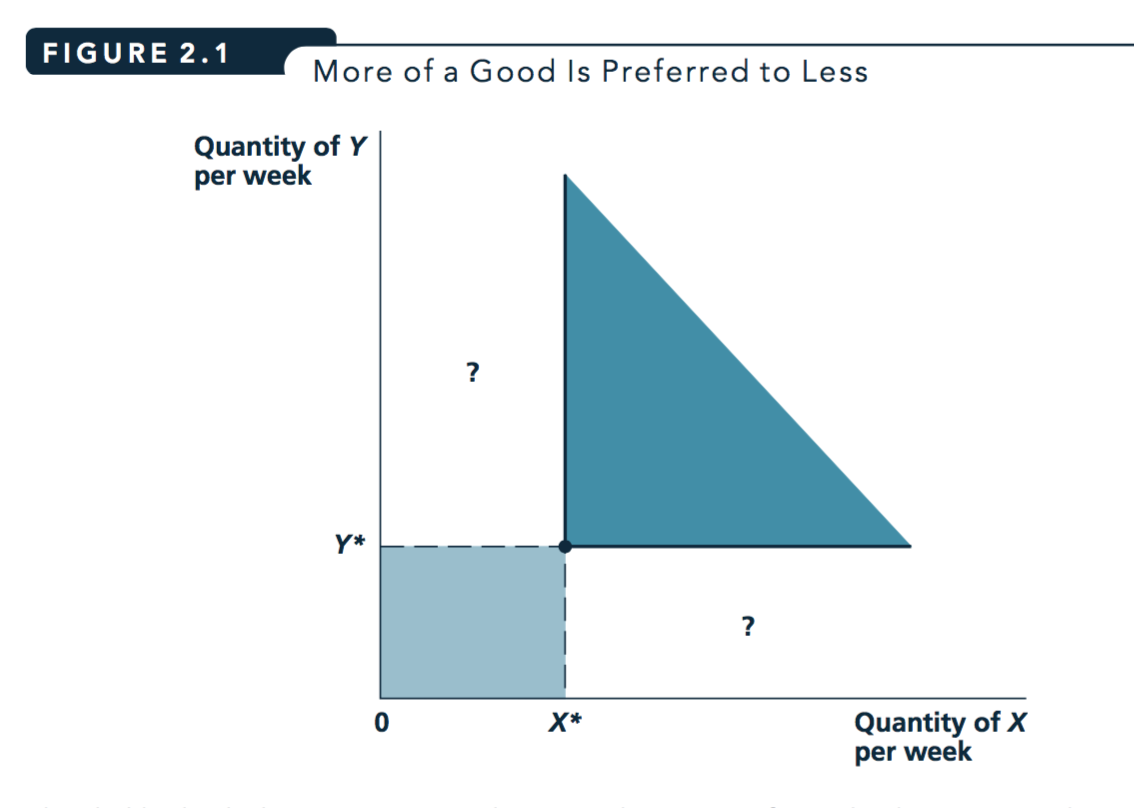
\includegraphics[width=0.8\linewidth]{picsfigs/moreisbetter} 

}

\end{figure}

\medskip

\emph{Draw this!}

\textcolor{gray}{ootnotesize{If the product is a 'bad' (e.g., pollution), redefine as the *absence} of the product*}

The darkly shaded area represents those combinations of X and Y that are
unambiguously preferred to the combination X*, Y*.

This is why goods are called `'goods''; individuals prefer having more
of any good rather than less.

Combinations of X and Y in the lightly shaded area are inferior to the
combination X*, Y*,

whereas those in the questionable areas may or may not be superior to
X*, Y*.

\end{block}

\end{frame}

\begin{frame}

\begin{block}{Who cares?}

\bigskip

\textbf{If people obey the first two assumptions (axioms),\(^\ast\) they
will make choices in a way consistent with maximising a (continuous)
\emph{utility} function}

\bigskip

\textcolor{gray}{*(and also 'continuity', which you can ignore for this module)}

silly to say people \emph{actually} consult a utility function.

instead `people behave as if they are maximizing utility functions';

similar to "people choose based on preferences that satisfy the above
assumptions.

Axioms stand directly behind `revealed preference' methods for measuring
how much people value

nonmarket goods, like clean air and national parks.

Also gives a vocabulary and a way to test for violations of this
consistency, and make alternate predictions

\end{block}

\end{frame}

\begin{frame}

\begin{figure}

{\centering 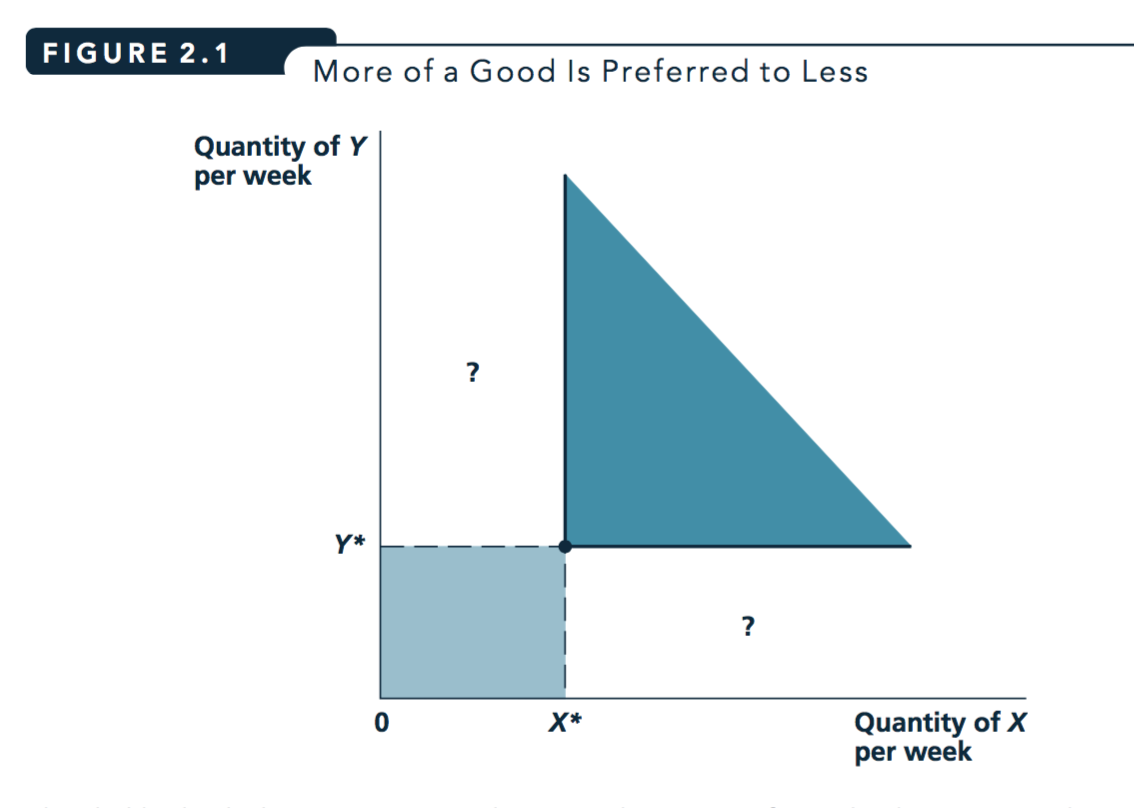
\includegraphics[width=0.6\linewidth]{picsfigs/moreisbetter} 

}

\end{figure}

\begin{itemize}
\tightlist
\item
  How can we compare the ``?'' areas? Which are preferred?
\end{itemize}

\begin{itemize}[<+->]
\tightlist
\item
  \(\rightarrow\) Compare utilities, depict using \emph{Indifference
  Curves}
\end{itemize}

LC: Here, put up indifference curve picture on the visualiser

\end{frame}

\begin{frame}{Voluntary trades and indifference curves}
\protect\hypertarget{voluntary-trades-and-indifference-curves}{}

\begin{description}
\tightlist
\item[Indifference curve]
A curve that shows all the combinations of goods or services that
provide the same level of utility
\end{description}

\bigskip

Formally (for 2 goods), the set of pairs of \(\{X,Y\}\) such that
\(U(X,Y)=c\) for some constant \(c\)

\bigskip

Recall ``level sets'' from math tools

\textcolor{red}{Warning:} Indifference curves help us \emph{depict}
utility functions; a single indifference curve is \emph{not} itself a
utility function!

\end{frame}

\begin{frame}

\begin{figure}

{\centering 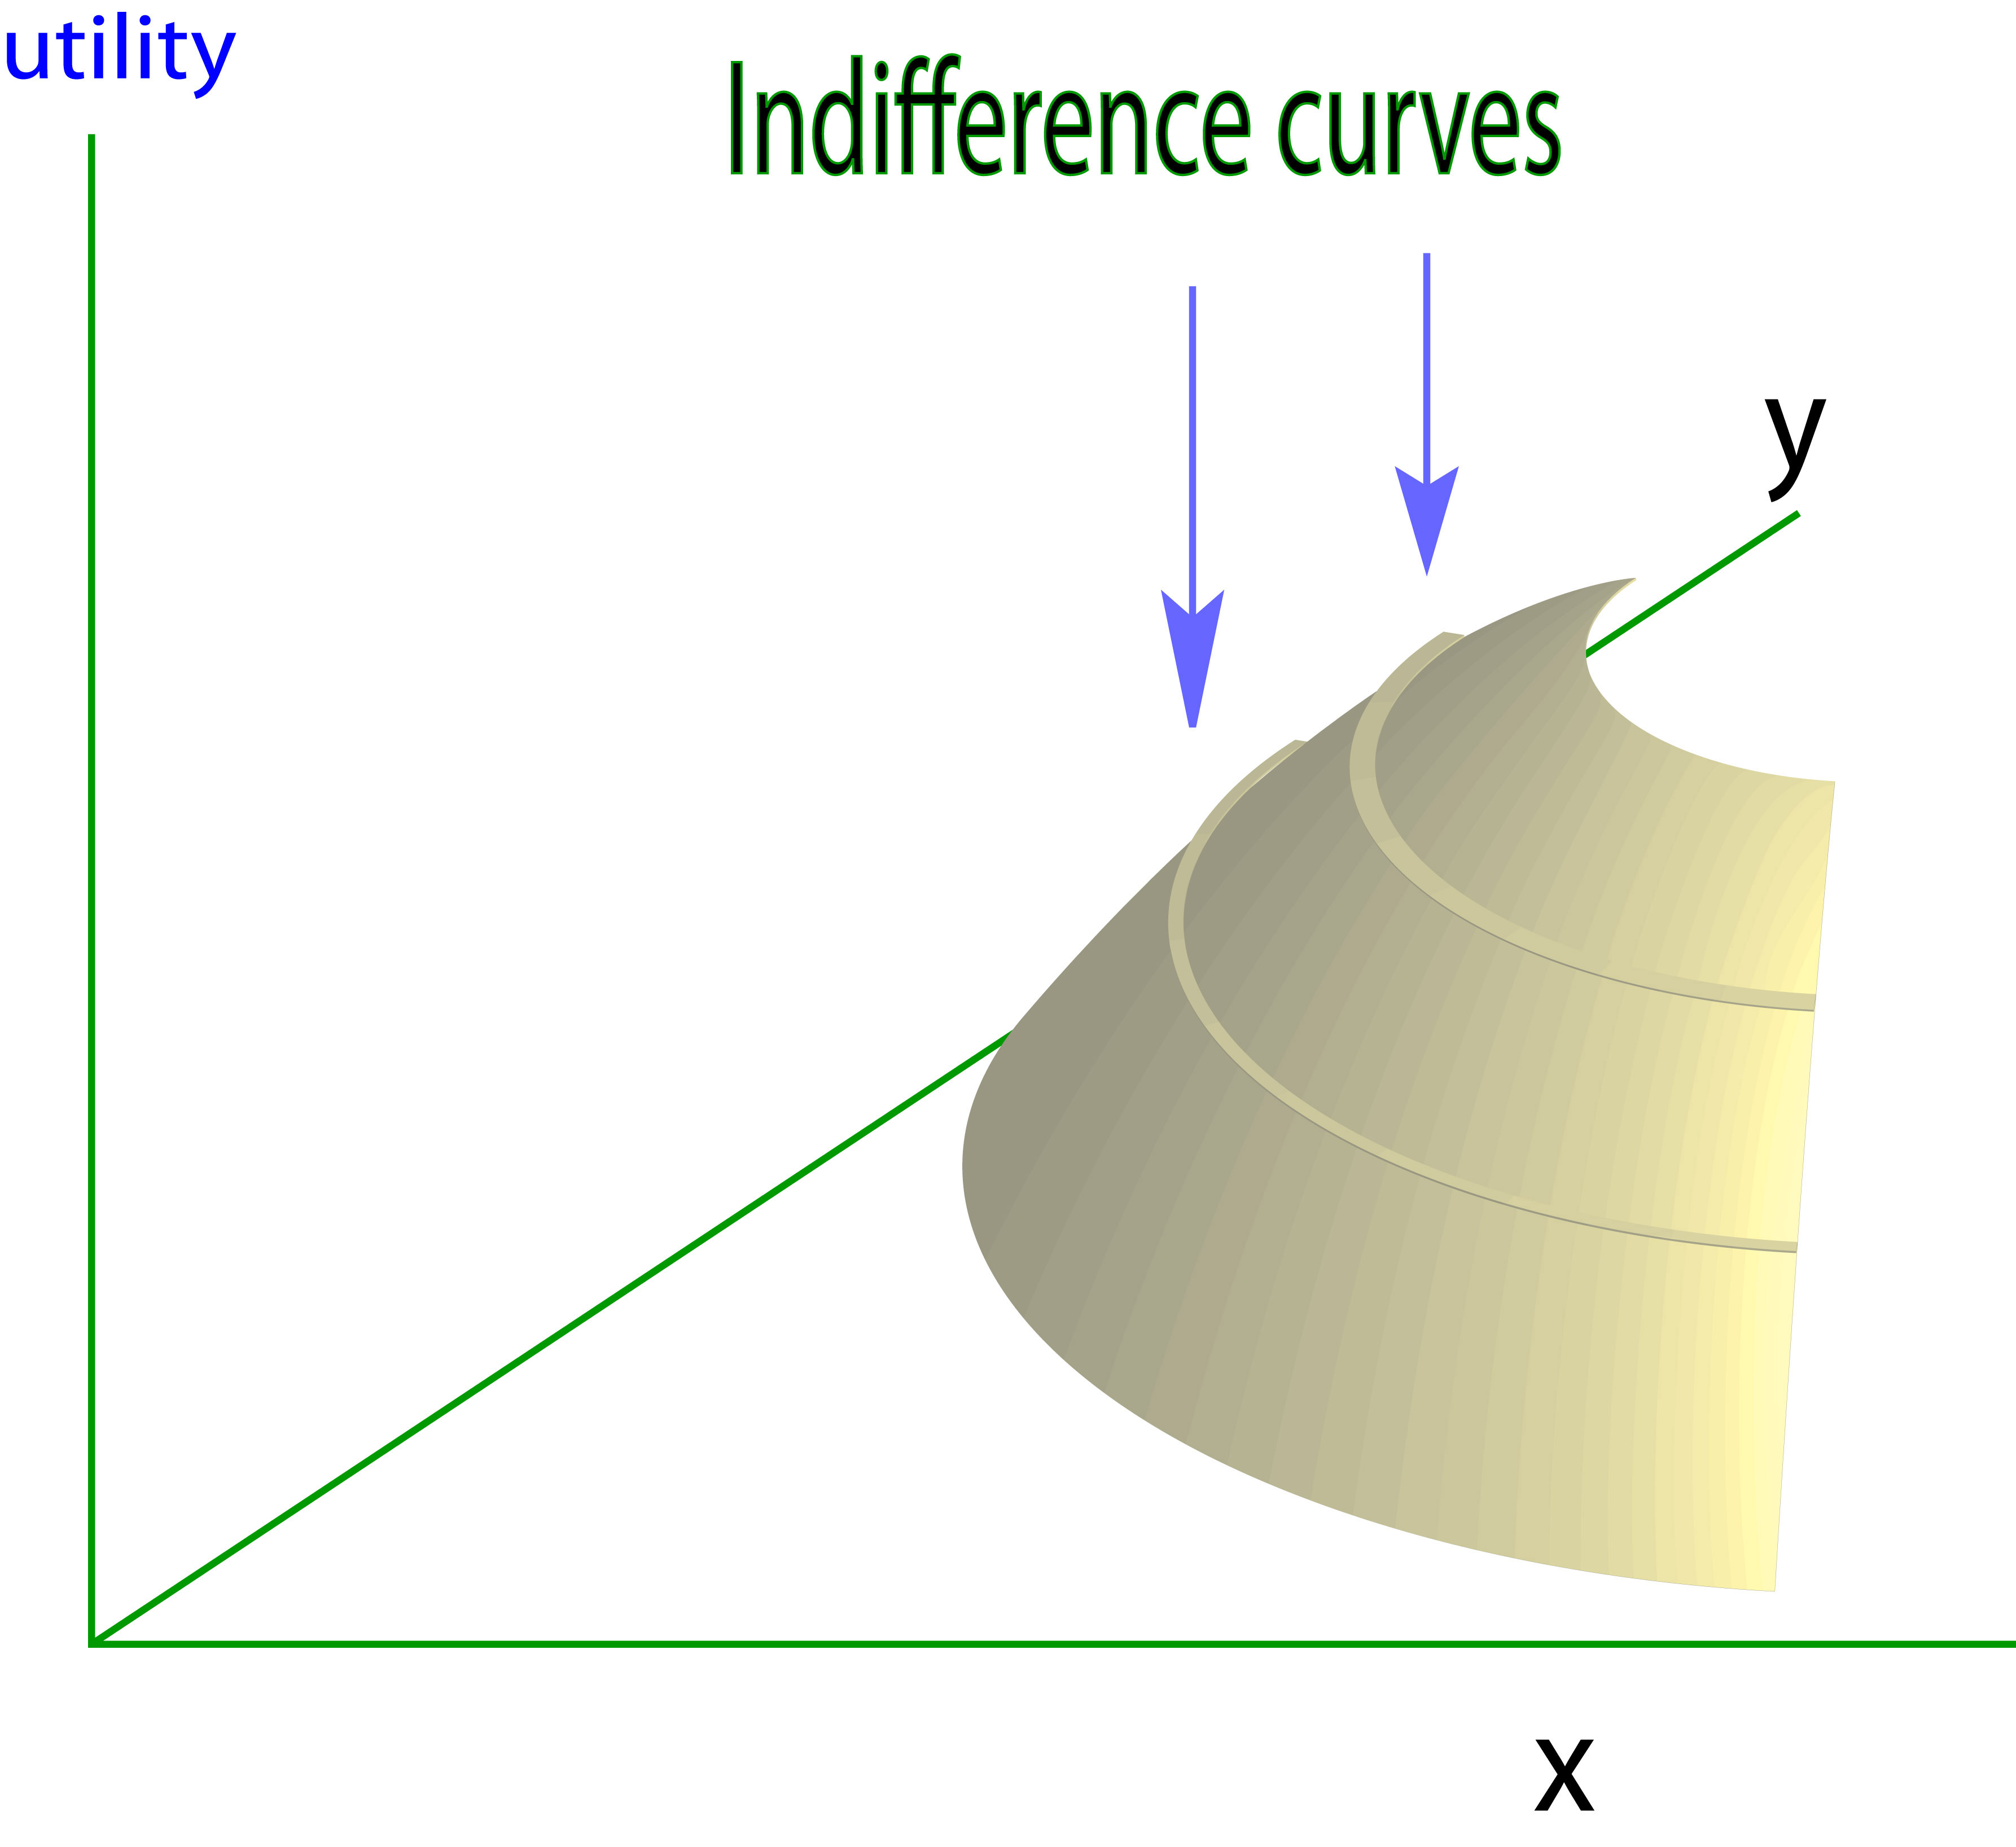
\includegraphics[width=0.7\linewidth]{picsfigs/indifcurves_util_together} 

}

\end{figure}

Credit: www2.econ.iastate.edu

\end{frame}

\begin{frame}

\begin{figure}

{\centering 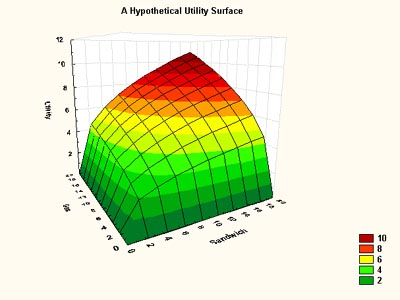
\includegraphics[width=0.8\linewidth]{picsfigs/indif_utility_2_400} 

}

\end{figure}

Credit: Frank's Economics on the web (MIT)

\end{frame}

\begin{frame}{Properties of indifference curves}
\protect\hypertarget{properties-of-indifference-curves}{}

\begin{figure}

{\centering 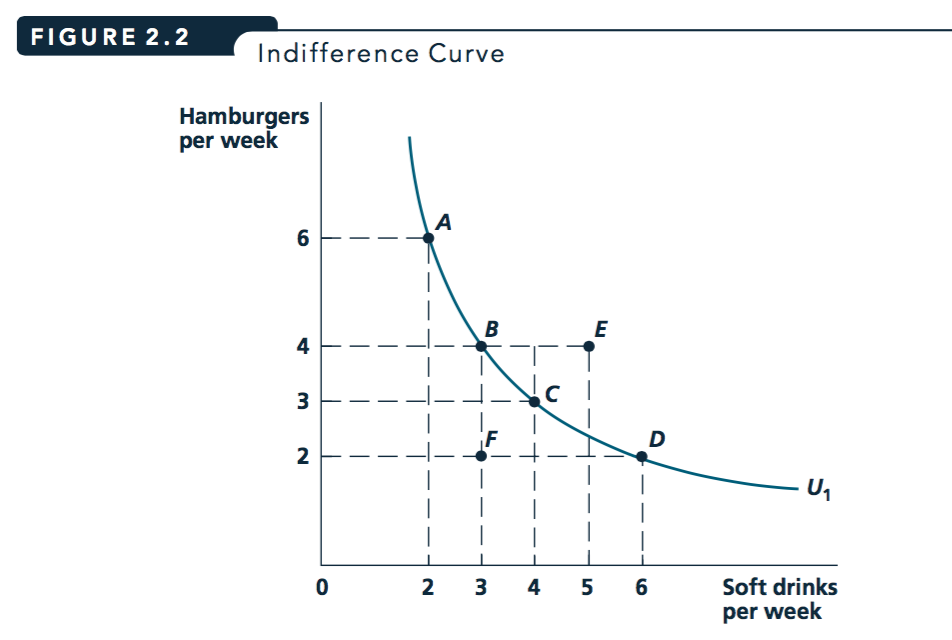
\includegraphics[width=0.8\linewidth]{picsfigs/indifccurve} 

}

\end{figure}

Suppose you are someone that likes hamburgers and soft drinks!

If this is too difficult, think of 2 healthy goods, like runner beans
and green tea.

Note that the \emph{period} of consumption; a day, a year, or a
lifetime, is not specified.

LC: draw/KEEP THIS ON THE BOARD

\textcolor{blue}{Rank order of preference/indifference between points A-E.}

Ans: \(E \succ A \sim B \sim C \sim D \succ F\)

\end{frame}

\begin{frame}

\begin{figure}

{\centering 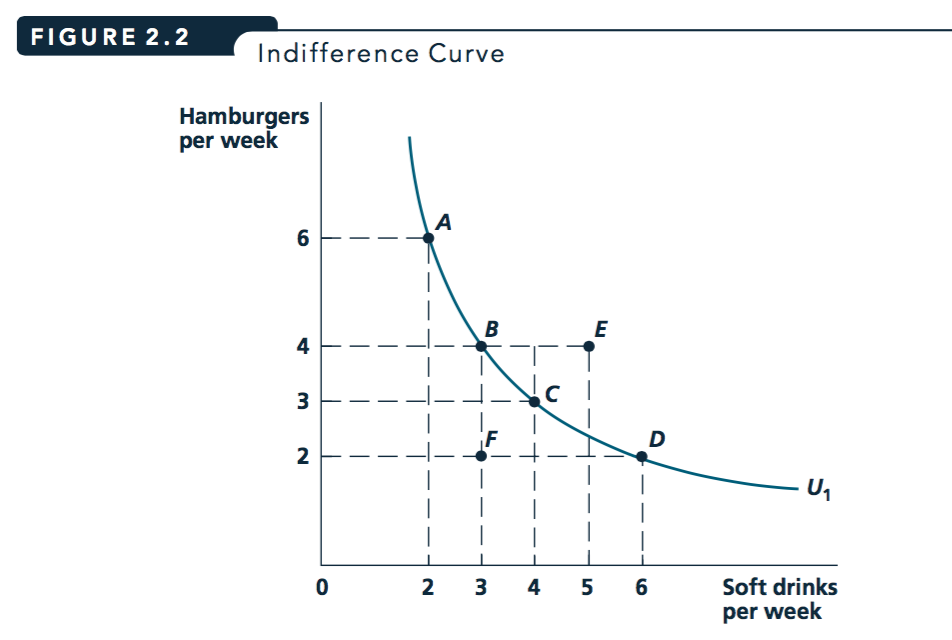
\includegraphics[width=13.22in,height=0.85\textheight]{picsfigs/indifccurve} 

}

\end{figure}

Q1: How do we know \(E \succ B\) ?

Q1: Has more soft drink, same hamburgers. Assumption 3: more preferred
to less.

Q: How do we know \(E \succ A\) ?

B indifferent to A because on same indifference curve

If \(E \succ A\) and \(B \sim A\) then \(E \succ A\) by transitivity of
the preferences, assumption 2.

\end{frame}

\begin{frame}

\textbf{Why `voluntary trade'? }

\begin{figure}

{\centering 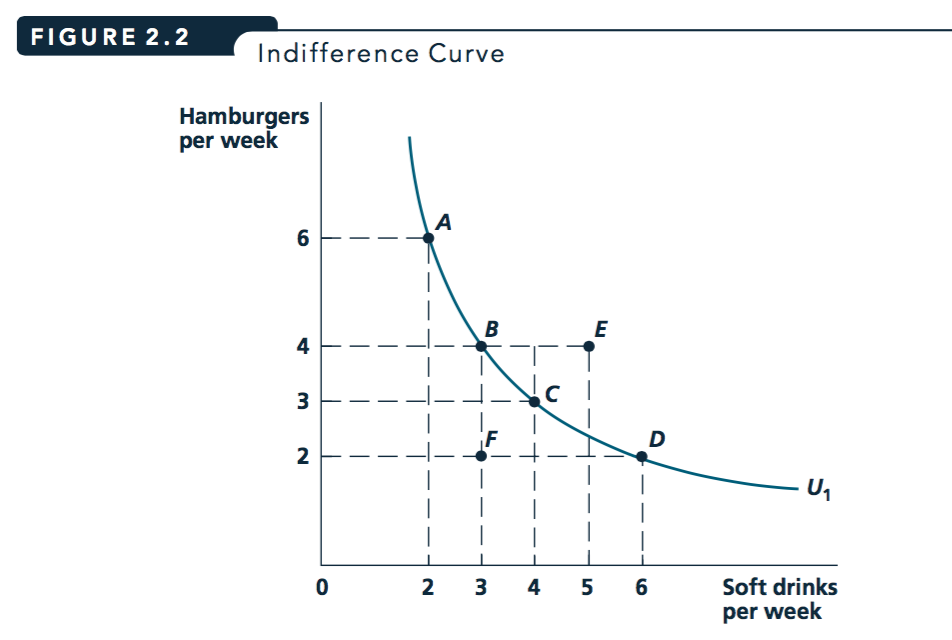
\includegraphics[width=0.8\linewidth]{picsfigs/indifccurve} 

}

\end{figure}

The indifference curve offers some intuition.

Individual ok giving up soda for hamburgers or v/v \emph{along}
indifference curve

A trade that put them \emph{above} the IC makes them `strictly' better
off

\emph{Consider if one individual had D and another A, and they had the
same preferences.}

Line between two bundles: all `convex combinations' of these,

In normal-speak, a partial share of each bundle.

Note with the same DMRS for both, trades along this line make both
better off;

the \emph{points} they would trade to depends on their bargaining power

\end{frame}

\begin{frame}{Marginal rate of substitution (MRS)}
\protect\hypertarget{marginal-rate-of-substitution-mrs}{}

MRS = Absolute value of slope of indifference curve

\bigskip

`Rate at which you're willing to forgo consuming (\(Y\)) to consume one
more (\(X\))'

2024, Adv, math: This slope will equal the negative of the \emph{ratio}
of the rate at which utility increases in each good (partial
derivative).

Intuition: giving up a certain utility from one good must be balanced by
an increase in utility from the other good.

\end{frame}

\begin{frame}

\emph{Back to fig 2.2 (board or visualiser)}

\begin{itemize}[<+->]
\tightlist
\item
  A to B: willing to give up 2 hamburgers to get 1 more soda.
\end{itemize}

\begin{itemize}[<+->]
\tightlist
\item
  \(\rightarrow\) slope \(-2\), \(MRS=2\)
\end{itemize}

\begin{itemize}[<+->]
\tightlist
\item
  From B to C? (think about it)
\end{itemize}

\begin{itemize}[<+->]
\tightlist
\item
  \ldots willing to give up 1 hamburger to get 1 more soda
  \(\rightarrow MRS =1\)
\end{itemize}

\begin{itemize}[<+->]
\tightlist
\item
  C to D?
\end{itemize}

\begin{itemize}[<+->]
\tightlist
\item
  \(MRS = \frac{1}{2}\)
\end{itemize}

Be careful: it is very easy to get the MRS inversed

Here this refers to arc slopes; however,

for continuous functions this gets closer and closer to the point slope

the smaller the arc

\begin{itemize}[<+->]
\tightlist
\item
  Note the decline: `diminishing MRS': may reflect \emph{satiation}
\end{itemize}

\end{frame}

\begin{frame}

\begin{block}{Preference for variety/balance}

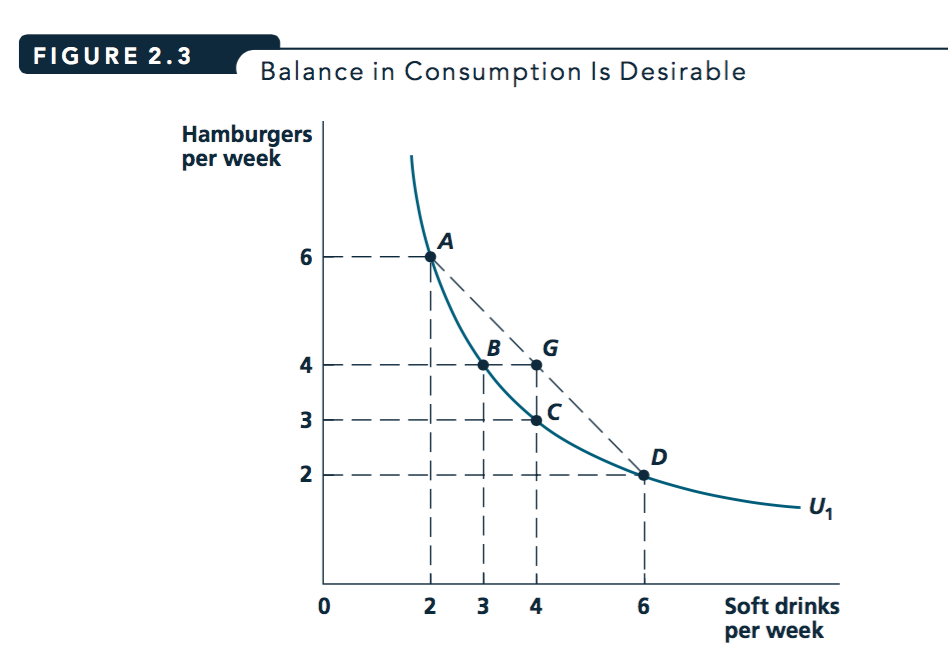
\includegraphics{picsfigs/indifcurvebalance.png}\\

Adv: this `preference for variety' is thought to hold for most
combinations of goods, most of the time, but perhaps not for all
pairings.

It tends to lead to easy-to-solve `interior solutions' where people may
consume some amount of each good, and have smooth reactions to price
changes.

Extreme of this is `necessity' goods.

LC: Adjust previous picture on visualiser/board

With an indifference curve with this shape (`convex')

any consumption bundle that represents a `mixture' between two equally
attractive extremes will be preferred to those extremes

E.g., if I like bundles A and D equally, I prefer a bundle of 1/3 of a
and 2/3 of D to either A or D.

\end{block}

\end{frame}

\begin{frame}

\begin{block}{Indifference curve map}

\begin{figure}

{\centering 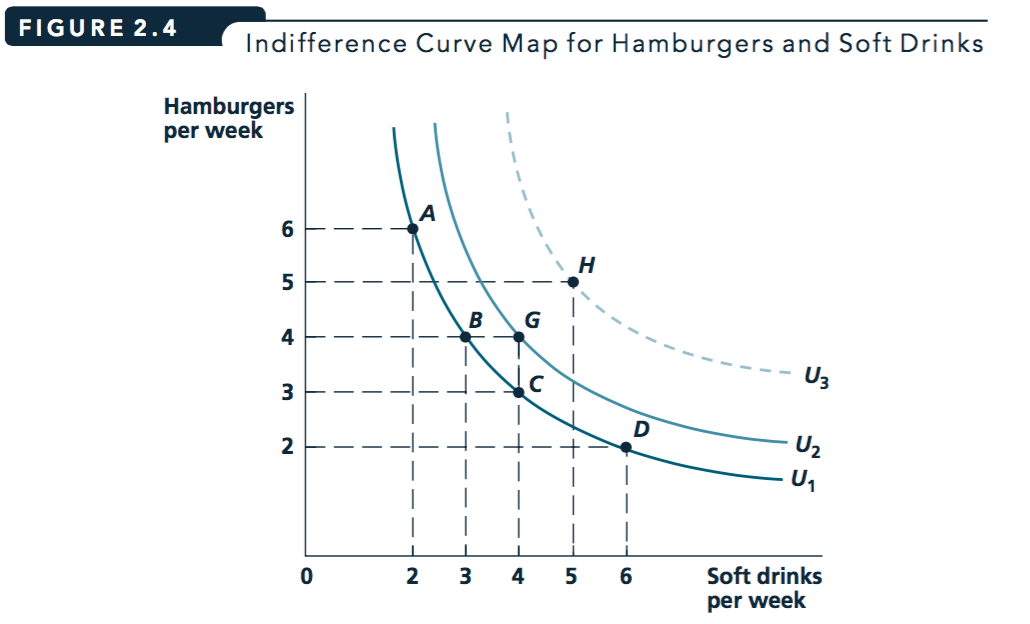
\includegraphics[width=0.9\linewidth]{picsfigs/indifcurvemap} 

}

\end{figure}

Indifference curves \textcolor{red}{never cross!}
\textcolor{red}{And are never upwards sloping!}

LC: Adjust previous picture on visualiser/board

Key principles: IC's never cross, never slope upwards, and they have
zero-thickness

\end{block}

\begin{block}{Illustrating particular preferences (NS fig 2.5)}

\begin{figure}

{\centering 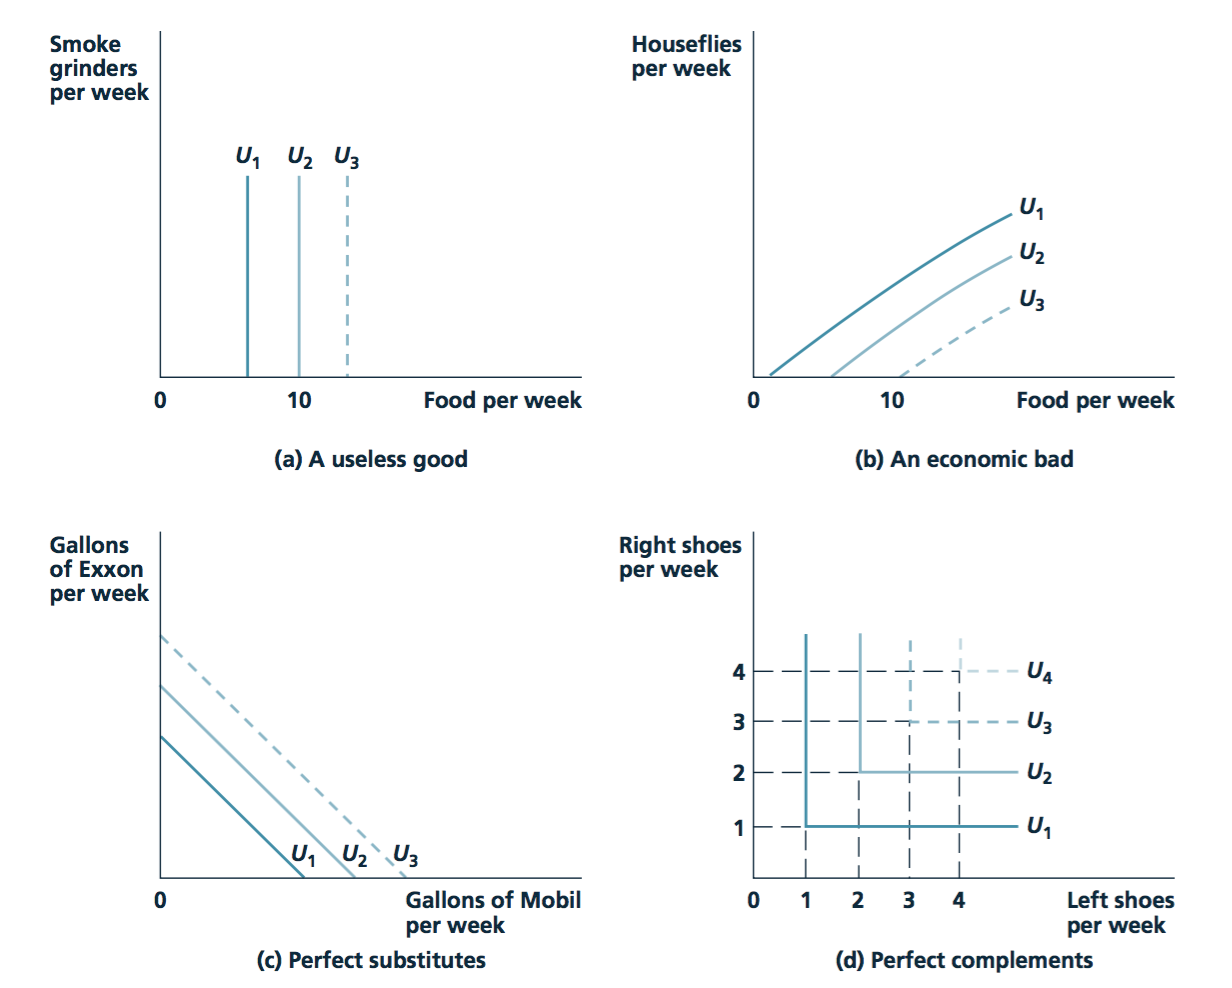
\includegraphics[width=0.7\linewidth]{picsfigs/particularpreferences} 

}

\end{figure}

Note, these preference violate some of the above assumptions and do not
exhibit diminishing MRS

\begin{itemize}
\item
  Smoke grinders are useless: violates `more is better'; can be ignored.
\item
  Houseflies are a \emph{bad}. (But housefly \emph{reduction} is a
  good).
\item
  Two types of petrol: \emph{perfect substitutes} (at 1:1); no
  preference for variety.
\item
  Left and right shoes are \emph{perfect complements} in 1:1
  proportions; no benefit to more of one without the other
\end{itemize}

\end{block}

\begin{block}{App 2.3: Product positioning in marketing (read at home,
see handout)}

\end{block}

\end{frame}

\begin{frame}{Definitions: Perfect substitutes and complements}
\protect\hypertarget{definitions-perfect-substitutes-and-complements}{}

\begin{description}
\item[Perfect substitutes]
Goods A and B are Perfect Substitutes when an individual's utility is
linear in these goods

when she is always willing to trade off A for B at a fixed rate (not
necessarily 1 for 1)
\end{description}

\end{frame}

\begin{frame}

\begin{description}
\item[Perfect complements]
Goods A and B are Perfect Complements when an individual only gains
utility from (more) A if she also consumes a defined (additional) amount
of B, and vice-versa
\end{description}

\bigskip

These goods are `enjoyed only in fixed proportions'.

e.g., left and right shoes (1-1) bicycle frames and wheels (1-2) or,
perhaps, baking powder and flour (1-40) for someone who only eats soda
bread.

We will give a specific functional form later.

\begin{block}{Choices are subject to constraints :(}

You cannot spend more than your (lifetime) income/wealth

\(\rightarrow\) \emph{budget constraint}.

Sorry \ldots{} maybe that's why they call Economics the dismal science

\begin{figure}[hb]
  \centering
    \begin{figure}
    
    {\centering 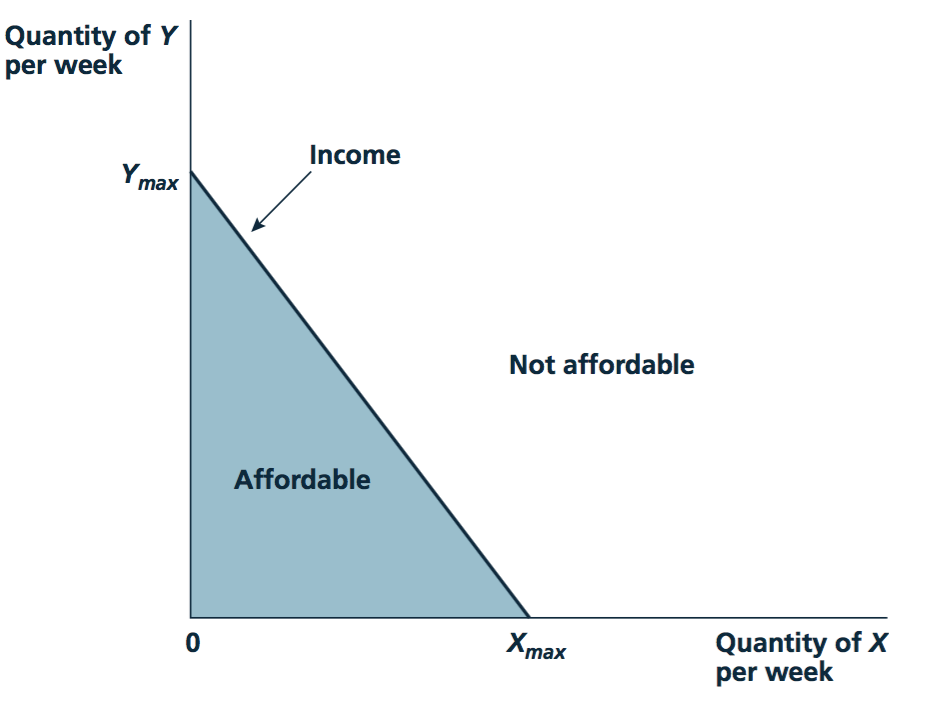
\includegraphics[width=0.75\linewidth]{picsfigs/budgetconstraint} 
    
    }
    
    \end{figure}
  \caption[Budget constraint for two goods]
   {Budget constraint for two goods, slope $-P_x/P_y$}
\end{figure}

Think `food' and `nonfood'.

Slope \(-Px/Py\): How much \(Y\) I must sacrifice to get another unit of
\(X\).

To get another \(X\) it costs me \(P_xX\), so the more costly is \(X\)
the more \(Y\) I must give up.

For each \(Y\) I give up I save \(P_Y\), so the more costly is \(Y\) the
more I can save by giving up 1 unit of it,

thus, the less I need to sacrifice of \(Y\) to get another unit of
\(X\).

Careful: it is very easy to get this slope ratio backwards!

However, I'll try not to make such errors too costly on the assessments.

\end{block}

\end{frame}

\begin{frame}

\begin{block}{Budget constraint algebra}

If I spend all my income
\textcolor{gray}{(I will do over a 'relevant lifetime')}:

Expenditure on X + Expenditure on Y = Income (I)

\[P_X X + P_Y Y = I \]

\begin{itemize}[<+->]
\tightlist
\item
  To see how \(Y\) trades off against \(X\), rearrange this to:
\end{itemize}

\[Y = -\frac{P_X}{P_Y} X + \frac{I}{P_Y}\]

\begin{itemize}[<+->]
\tightlist
\item
  Intercept \(\frac{I}{P_Y}\): amount of Y you can buy if you only buy Y
\item
  Slope \(-\frac{P_X}{P_Y}\): how much Y you must give up to get another
  X
\end{itemize}

Work on making sure you can calculate the slope and intercept,

what they mean, and have intuition for why the slope has this formula.
See `micro quiz 2.3'.

\end{block}

\end{frame}

\begin{frame}{Utility maximization}
\protect\hypertarget{utility-maximization}{}

\begin{figure}

{\centering 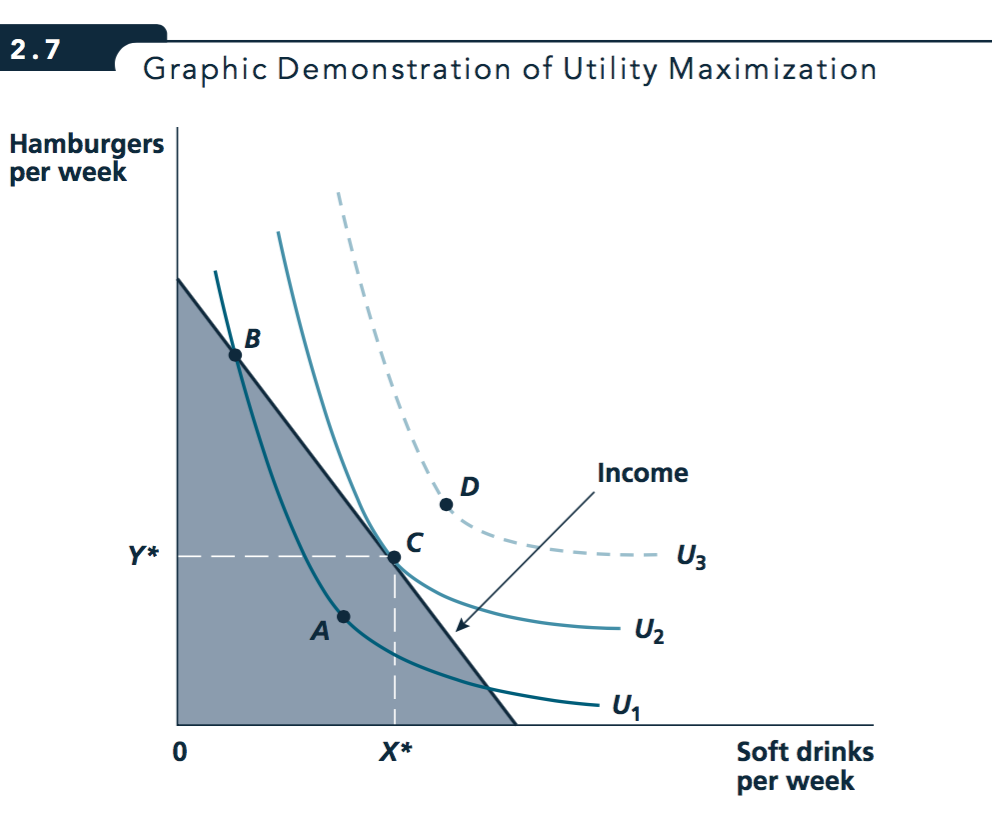
\includegraphics[width=0.75\linewidth]{picsfigs/utilmax} 

}

\end{figure}

LC: Depict on visualiser/board

\begin{itemize}
\item
  Can choose any point in shaded area, want to get to highest
  indifference curve\\
\item
  How do we know A is suboptimal? B? Points between B and C?
\item
  Will choose point C, yielding utility \(U_2\)\\
\item
  What is special about point C?\\
\item
  It's the point of \emph{tangency} between the budget constraint and an
  indifference \emph{curve}\\
\item
  Point where the slope of budget constraint = slope of indifference
  curve
\end{itemize}

\end{frame}

\begin{frame}

\begin{figure}

{\centering 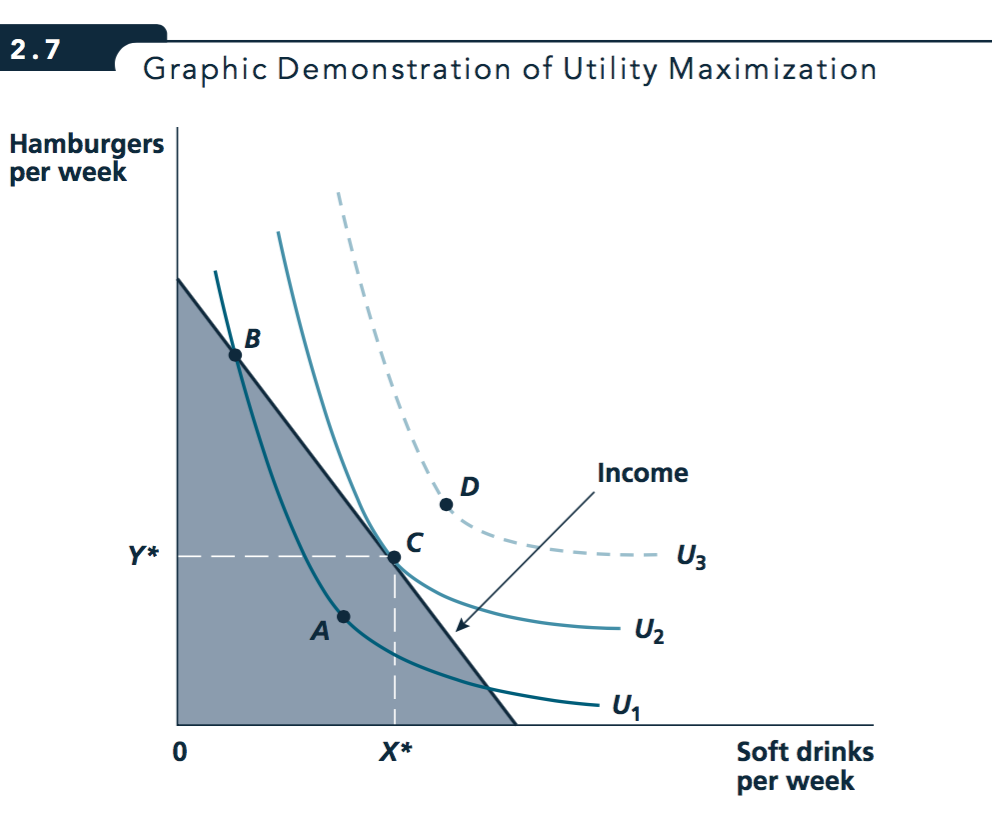
\includegraphics[width=0.5\linewidth]{picsfigs/utilmax} 

}

\end{figure}

\bigskip

\emph{If} slope budget constraint = slope indifc curve at point X,Y
\(\rightarrow\) \[P_X/P_Y = MRS(X,Y)\]

As both slopes are negative both negative signs cancel out, leaving this
condition.

\begin{itemize}[<+->]
\tightlist
\item
  \textcolor{red}{Warning:} This equality holds \emph{at an optimal
  choice}; it doesn't hold everywhere.
\end{itemize}

\end{frame}

\begin{frame}

\textbf{At an optimal consumption choice}
\textcolor{gray}{(given above assumptions)}

\begin{itemize}
\tightlist
\item
  Consume all of income;
  \textcolor{gray}{locate *on* budget line; follows from 'more is better'}
\end{itemize}

\begin{itemize}[<+->]
\tightlist
\item
  Psychic tradeoff (MRS) equals market tradeoff (\(P_X/P_Y\))
  \textcolor{gray}{if consuming both goods}
\end{itemize}

This holds for all goods where you consumed a positive amount, assuming
`convex preferences'.

\end{frame}

\begin{frame}

Psychic tradeoff (MRS) equals market tradeoff (\(P_X/P_Y\))
\textcolor{gray}{if consuming both goods}

\bigskip

\emph{Key intuition:}

\begin{itemize}[<+->]
\tightlist
\item
  If I can give up X for (buy less X, get more Y) at some rate, and the
  \emph{benefit} I get from doing this is at a \emph{different} rate,
\end{itemize}

\begin{itemize}[<+->]
\tightlist
\item
  \ldots then I can make myself better off.
\end{itemize}

\begin{itemize}[<+->]
\tightlist
\item
  Thus the original point could not have been optimal.
\end{itemize}

Think about this carefully; it is a key method of proving things in
economic theory.

See example in handout and practice question there

\end{frame}

\begin{frame}

\begin{block}{More insight (mathy: ignore if this freaks you out)}

Recall \(U=U(X,Y)\).

\[U_X(X,Y) := MU_X(X,Y)\]

\medskip

\emph{Derivative w/ respect to X: rate utility increases if we add a
little X, holding Y constant}

\ldots{} Similarly for \(MU_Y\).

\begin{itemize}[<+->]
\tightlist
\item
  MRS: `how much Y would I be willing to give up to get a unit of X'?
\end{itemize}

\begin{itemize}[<+->]
\tightlist
\item
  Ans: Depends on marginal benefit of each \ldots{} we can show
  \(MRS(X,Y)=\frac{MU_{X}}{MU_{Y}}\)
\end{itemize}

Intuition: the more valuable a little more X is to me -- the higher is
MU\_X --

the more Y I am willing to give up to get it. That is why MU\_X is in
the numerator

See derivation in handout if interested

\end{block}

\end{frame}

\begin{frame}

Rearranging the utility maximising condition yields more intuition:

\[P_X/P_Y = MRS = MU_X/MU_Y\]

(at each consumption point X,Y)

\medskip

\begin{itemize}[<+->]
\tightlist
\item
  \[\frac{MU_X}{P_X} = \frac{MU_Y}{P_Y}\]
\end{itemize}

\begin{itemize}[<+->]
\tightlist
\item
  Same `bang for each buck' (\textcolor{red}{if} optimising)
\end{itemize}

If this didn't hold true and you were spending on both goods,

you would be paying `more per util' for one good than the other,

and thus should reallocate to that other good.

The more valuable a little more X is to me at that point

-- the higher is MU\_x -- the more Y I'm willing to give up to get it.

That is why MU\_x is in the numerator. The more valuable a bit more Y is
at that point -- the higher is MU\_y -- the less Y I am willing to give
up to get a bit more X.

That is why MU\_y is in the denominator

\begin{block}{Caveat on `corner solutions'}

\begin{itemize}
\tightlist
\item
  If you are consuming \emph{both goods} and optimising,
  \(P_X/P_Y = MRS = MU_X/MU_Y\) must hold
\end{itemize}

\bigskip

\textcolor{gray}{Advanced: This is a 'necessary but not sufficient condition', sufficient if DMRS everywhere}

Same condition applies to each good you are consuming a positive amount
o \bigskip f

\bigskip

\textcolor{red}{But...}

\end{block}

\end{frame}

\begin{frame}

\begin{block}{But\ldots{}}

\begin{figure}

{\centering 
\includegraphics[width=0.8\linewidth]{picsfigs/chiapet} 

}

\end{figure}

\end{block}

\end{frame}

\begin{frame}

\begin{itemize}
\tightlist
\item
  If you are consuming both goods and optimising,
  \(P_X/P_Y = MRS = MU_X/MU_Y\) must hold
\end{itemize}

\begin{itemize}[<+->]
\tightlist
\item
  But you might consume \emph{none} of some good (say X):
\end{itemize}

\begin{itemize}[<+->]
\tightlist
\item
  if even with \emph{no} X, \(MU_X/P_X<MU_Y/P_Y\), the marginal utility
  of the first unit `per pound' is lower
\end{itemize}

\end{frame}

\begin{frame}

\begin{figure}

{\centering 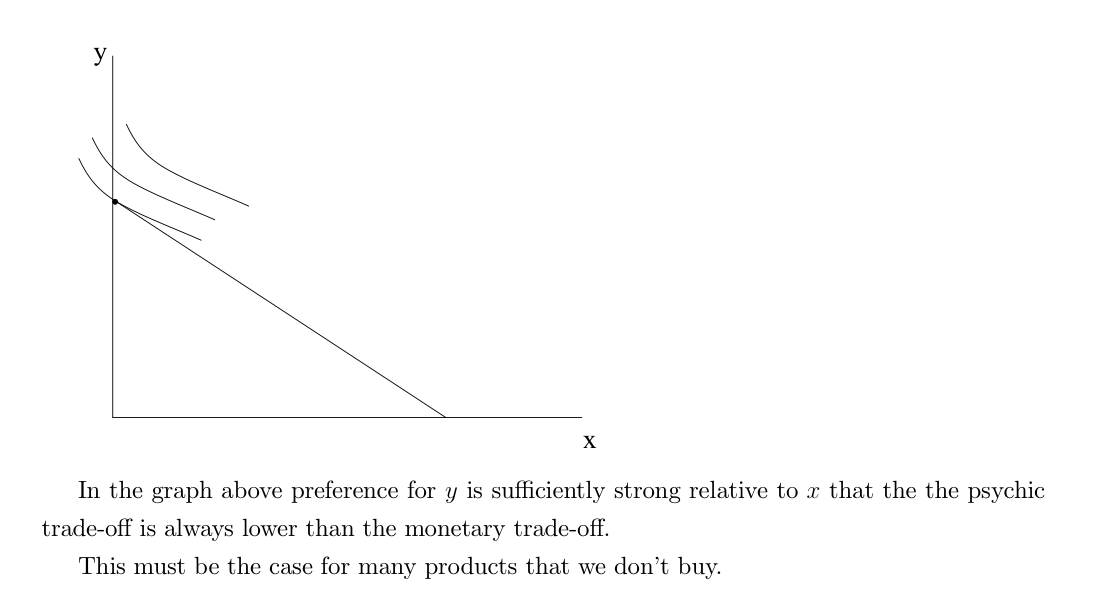
\includegraphics[width=1\linewidth]{picsfigs/goodwedontbuy} 

}

\end{figure}

\end{frame}

\begin{frame}{App 2.4: ticket scalping}
\protect\hypertarget{app-2.4-ticket-scalping}{}

\begin{figure}

{\centering 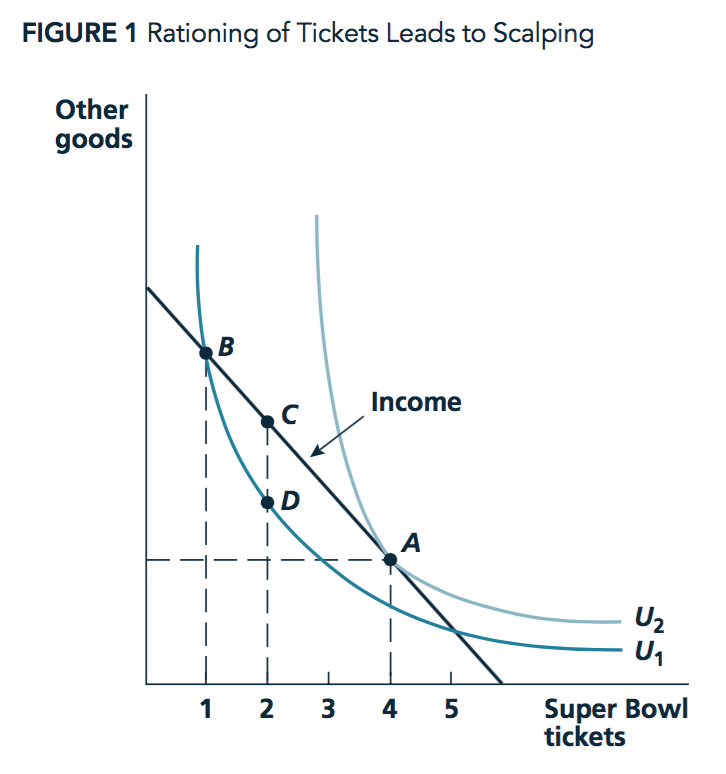
\includegraphics[width=0.6\linewidth]{picsfigs/scalping} 

}

\end{figure}

\begin{itemize}
\item
  tickets are rationed: one per customer
\item
  Constraint \(\rightarrow\) Lower utility; would choose A if
  unconstrained
\item
  budget line not tangent to indifference curve, slopes not equal
\item
  Would be better off buying more tickets, but cannot
\item
  Would be willing to buy additional ticket at full price (move to point
  C)
\item
  Willing to pay \emph{more} than full price for second ticket

  \begin{itemize}
  \tightlist
  \item
    could give up up to an additional C-D of goods for ticket 2 and
    still be as well off
  \end{itemize}
\end{itemize}

\begin{itemize}
\item
  Adv: Tough questions:

  \begin{itemize}
  \item
    Why would NFL institute this rule?
  \item
    Who benefits? (Maybe poor consumers?)
  \item
    Why do people see scalping as unfair?
  \item
    Is there ever a justification to forbid a transaction between 2
    consenting parties?
  \end{itemize}
\end{itemize}

\begin{block}{App 2.5: What's a rich uncle's promise worth?}

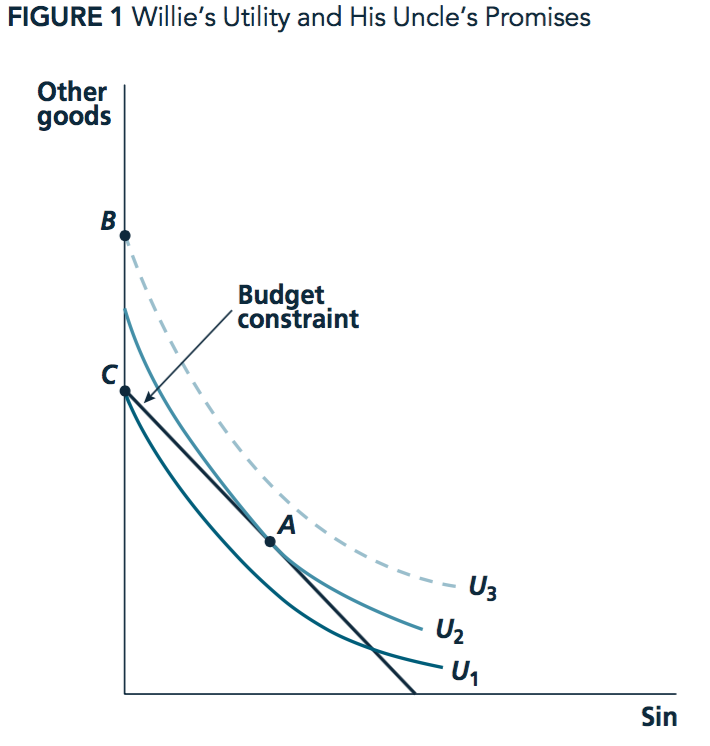
\includegraphics{picsfigs/williesuncle.png}\\

\begin{itemize}
\item
  Willie would choose point A, but paid \$5k to abstain, would get him
  to point B, gain \(U_3\)
\item
  Graphically, how much \$ would have been enough to compensate for
  abstaining?
\item
  Hard question, foreshadowing: How much would Willie need to be paid to
  get him to \(U_3\) \emph{without} the restriction?
\item
  Is this more or less than \$5k?
\end{itemize}

\end{block}

\end{frame}

\begin{frame}{Using the model of choice}
\protect\hypertarget{using-the-model-of-choice}{}

\begin{enumerate}
\tightlist
\item
  Why do people spend their money on different things?
\item
  What do different preferences/indifference curves imply for choices?
\end{enumerate}

LC: Move to PowerPoint slides here for graphical illustration,

beginning with `Utility Maximization: A Graphical View' and going
through `different types of goods'

\begin{itemize}
\item
  what indicates each persons' preference for one good over the other?

  \begin{itemize}
  \item
    The shape of the indifference curve.
  \item
    The flatter (steeper) the indifference curve the stronger the
    preference for the good on the Y-axis (X-axis)
  \end{itemize}
\end{itemize}

\end{frame}

\begin{frame}

\emph{Move to ppt slides here beginning with `Utility Maximization: A
Graphical View'}

todo: integrate into main presentation

\end{frame}

\begin{frame}{Algebraic/numerical examples}
\protect\hypertarget{algebraicnumerical-examples}{}

\end{frame}

\begin{frame}

Consider: are these `perfect substitutes' for someone who wants
caffeine, but has no taste buds?

\begin{figure}

{\centering 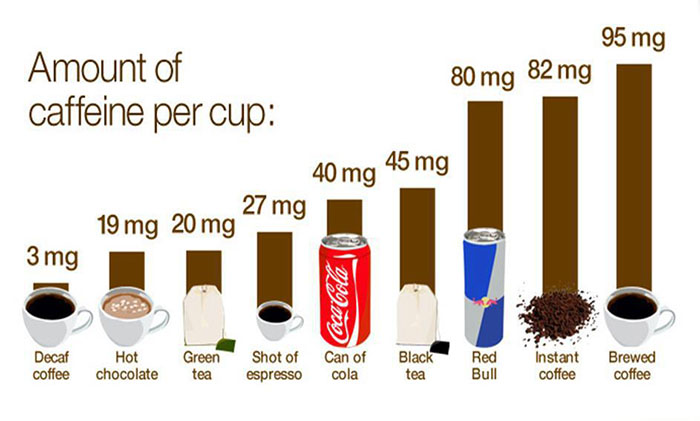
\includegraphics[width=0.9\linewidth]{picsfigs/amount-of-caffeine-in-drinks} 

}

\end{figure}

\end{frame}

\begin{frame}

\begin{block}{Perfect substitutes, but not identical, e.g.,}

This may be confusing.

By `perfect substitutes' we mean pairs of goods for which \emph{some
amount} of one is always valued the same as \emph{some amount} of the
other,

and this proportion is always the same.

An easy example: I might always be indifferent between three pints of
mild ale and two pints of strong ale,

if they have the same total alcohol content and I only want to get
tipsy.

\[U(X,Y)=4X+3Y\]

Rates each increase utility per-unit (derivative) are constant:
\(MU_X = 4\), \(MU_Y = 3\)

So (for perfect substitutes) buy the one that increases it more
*per-\pounds*

\end{block}

\end{frame}

\begin{frame}

\textbf{With perfect substitutes: `Bang for the buck' rule}

\[U(X,Y)=4X+3Y\]

\bigskip

\begin{itemize}
\tightlist
\item
  Compare \(MU_X/P_X\) to \(MU_Y/P_Y\)
\end{itemize}

\begin{itemize}
\item
  Here, if \(4/P_X > 3/P_Y\), then buy X
\item
  if \(4/P_X < 3/P_Y\), then buy Y;
  \textcolor{gray}{(if equal, buy either)}
\item
  Rearranging, if \(P_X < 4/3 P_Y\), buy X \ldots{} etc.
\end{itemize}

\textcolor{red}{Warning:} If \emph{not} perfect substitutes, MU ratios
depend on consumption levels.

\end{frame}

\begin{frame}

\begin{block}{Perfect complements}

AKA `Leontief preferences'

Lecture question: come up with an example

Mathematical function example:\\

\[U(X,Y)=min(2X,Y)\]

\textcolor{gray}{E.g., X: bicycle frames, Y: wheels.}

\bigskip

\textcolor{red}{Warning:} this min function looks backwards, but it's
correct; see notes

\begin{itemize}
\tightlist
\item
  Shortcut: figure out the proportions it will be consumed in

  \begin{itemize}
  \tightlist
  \item
    determine cost of `1 bundle of the combo' at given prices
  \item
    \ldots{} then buy as many such bundles as you can afford
  \end{itemize}
\end{itemize}

``Min'' function just takes the smaller of the arguments

to max this (not waste money), set the arguments to `min' equal, here
2X=Y

You should be able to do this without having taken economics.

Suppose you were given \pounds100 and asked to spend it to make as many
sausages-with-baps as possible.

No one can eat a sausage without a bap, nor vice-versa. Sausages come in
packs of 4, and baps come in packs of 8. How many packs of each will you
buy,

Supposing both types of packs cost \pounds1 each?

\end{block}

\end{frame}

\begin{frame}

\begin{block}{Middle-ground (*)}

A Cobb-Douglas example

\[ U(X,Y)=\sqrt(XY) \]

LC: We are `allowed' to square the whole thing to simplify the problem.
Why?

\[MU_X = \frac{\partial}{\partial X} (XY)^{1/2} = \frac{1}{2} (Y/X)^{1/2}\]

\[MU_Y =  \frac{1}{2} (X/Y)^{1/2}\]

General Cobb-Douglas: \(U(X,Y)=X^a Y^b\) for a, b positive constants

\bigskip

\emph{Here, amount of Y you'd give up to get a unit of X:}

\[MRS(X,Y)= MU_X/MU_Y = Y/X\]

MU\_X is the slope of U(X,Y) in X at a particular point, i.e., the
(partial) derivative with respect to X

The last equality comes from this \emph{particular} function; it is not
always Y/X.

\footnotesize\{Check reasonable: The more Y I've , the more Y I'd give
up to get another X :)\}

This slope is derived through calculus.

Adv, maths:

MU\_X is the slope of U(X,Y) in X at a particular point, i.e., the
(partial) derivative with respect to X

\(MU_X = \frac{\partial</aside>{\partial X} (XY)^{1/2} = \frac{1}{2} (XY)^{-1/2}Y = \frac{1}{2} (Y/X)^{1/2}\)

Similarly, \(MU_Y = \frac{1}{2} (X/Y)^{1/2}\).\}

\end{block}

\end{frame}

\begin{frame}

\emph{\ldots Cobb-Douglas ctd}

\[MRS(X,Y)= MU_X/MU_Y = Y/X\]

Here utility-maximization requires, at optimal choices of X and Y:
\[MRS(X,Y)= Y/X = P_X/P_Y\]

Check it makes sense.

As P\_X increases the right-hand-side (RHS) increases,

and so to increase the LHS I must increase the units of Y consumed,

and thus decrease the units of X consumed

I say `here' because we now have nice convex indifference curves with
`normal' slopes,

unlike for perfect complements or substitutes.

The more of one good you have the less you value it relative to the
other good (unlike perfect substitutes)

but you still value more of it somewhat (unlike for perfect complements)

For any price ratio, find ratio of Y \& X.

With prices and income, \(I\), find consumption of X \& Y.

Rearranging optimization condition:

\[Y P_Y = X P_X\]

Class question- What is weird about this? Ans: You always spend the same
\emph{amount} on each good, no matter the price

(Note, that doesn't mean the same number of units)

This `constant expenditure shares' are a characteristic of Cobb-Douglas
functions that limit their usefulness and realism

\end{frame}

\begin{frame}

Optimization condition for \textcolor{red}{this particular} utility
function:

\[Y P_Y = X P_X\]

Combining this with the budget constraint \[P_X X + P_Y Y = I\]

solve for X \& Y, as fncns of prices \& income (see notes)
\(\rightarrow\)

\medskip

\[Y = I/(2P_Y)\] \[X = I/(2P_X)\]

Rearranging the optimization condition, \(Y = X P_X/P_Y\).\\
From the b.c., \(X = (I - P_Y Y)/P_X\).\\
Substituting in for \(Y\) yields
\(X = (I - P_Y(X P_X / P_Y))/P_X = I/P_X - X\)\\
\(\rightarrow 2X = I/P_X \rightarrow X = I/(2P_X)\)\\
\(X P_X = I / 2 \rightarrow\) always spend half your income on X.\\
Adv: You can solve for the optimal \(Y\) by `symmetry': as utility\\
and budget constraint are symmetric everything we said holds replacing X
with Y.\\

\end{frame}

\begin{frame}{Second problem set: covers NS chapter 2 (and chapter 3) --
see bottom}
\protect\hypertarget{second-problem-set-covers-ns-chapter-2-and-chapter-3-see-bottom}{}

Preferences, Utility, Consumer optimization,

\bigskip

individual and market demand curves.

This is a very large problem set (others are smaller).

\end{frame}

\begin{frame}

\end{frame}

\end{document}
